% FENG 498 Poster - Warehouse Layout Optimization (beamerposter)
% A0 portrait. Build: pdflatex poster.tex (x2)
\documentclass[final]{beamer}
\usepackage[size=a0,orientation=portrait,scale=1.25]{beamerposter}
\usepackage[T1]{fontenc}
\usepackage[utf8]{inputenc}
\usepackage{graphicx}
\usepackage{amsmath}
\usepackage{booktabs}
\usepackage{colortbl}
\usepackage[most]{tcolorbox}
\usepackage{ragged2e}
\graphicspath{{figs/}}

% ---- palette ----
\definecolor{senavy}{RGB}{12,46,74}
\definecolor{seteal}{RGB}{0,122,138}
\definecolor{segreen}{RGB}{52,168,83}
\definecolor{seink}{RGB}{28,36,44}
\definecolor{sebg}{RGB}{237,241,245}

% ---- look ----
\setbeamercolor{background canvas}{bg=sebg}
\setbeamercolor{block title}{bg=senavy,fg=white}
\setbeamercolor{block body}{bg=white,fg=seink}
\setbeamerfont{block title}{size=\Large,series=\bfseries}
\setbeamertemplate{navigation symbols}{}
\setbeamertemplate{caption}{\raggedright\insertcaption\par}
\setbeamertemplate{itemize items}{\textcolor{segreen}{\textbullet}}

% rounded block with a slim shadow
\setbeamertemplate{block begin}{
  \begin{tcolorbox}[enhanced,colback=white,colframe=senavy,boxrule=0pt,
    arc=5mm,left=8mm,right=8mm,top=0mm,bottom=6mm,
    drop fuzzy shadow=black!22,
    title=\strut\insertblocktitle,coltitle=white,
    colbacktitle=senavy,fonttitle=\Large\bfseries,
    attach boxed title to top left={xshift=6mm,yshift=-5mm},
    boxed title style={colframe=senavy,arc=3mm,boxrule=0pt}]
}
\setbeamertemplate{block end}{\end{tcolorbox}\vspace{14mm}}

% ---- header ----
\setbeamertemplate{headline}{
  \begin{beamercolorbox}[wd=\paperwidth]{headline}
  \colorbox{senavy}{\begin{minipage}[c][0.155\paperheight][c]{\paperwidth}
  \centering
  \begin{minipage}{0.13\paperwidth}
    
\includegraphics[width=\linewidth]{ieu_logo}
  \end{minipage}\hfill
  \begin{minipage}{0.80\paperwidth}
    \raggedright
    {\color{white}\bfseries\fontsize{72}{78}\selectfont WAREHOUSE LAYOUT OPTIMIZATION\par}
    \vspace{6mm}
    {\color{segreen!55!white}\bfseries\LARGE A Simulation Study of Storage
    Assignment Policies at the Schneider Electric Manisa Plant Warehouse\par}
    \vspace{8mm}
    {\color{white}\large Deniz Etensel \,$\cdot$\, Deniz Ege Memeto\u{g}lu
    \,$\cdot$\, Nehir Konyar \,$\cdot$\, Elif Bostanc\i{} \,$\cdot$\,
    Yi\u{g}it Ka\c{c}ar \,$\cdot$\, S\"umeyra Pul\c{c}a \quad$|$\quad
    Supervisor: Dr.\ Oktay Karaba\u{g}\par}
  \end{minipage}\hspace{0.01\paperwidth}
  \end{minipage}}
  \end{beamercolorbox}
  \vspace{10mm}
}

% stat card
\newtcolorbox{statcard}[1]{enhanced,colback=white,colframe=#1,boxrule=1.5mm,
arc=5mm,left=2mm,right=2mm,top=4mm,bottom=4mm,halign=center,
drop fuzzy shadow=black!25,valign=center,height=11cm}

\newcommand{\bignum}[1]{\color{senavy}\bfseries\fontsize{96}{96}\selectfont #1}

\begin{document}
\begin{frame}[t]

% ===== headline stat cards =====
\begin{columns}[t,totalwidth=\textwidth]
\begin{column}{0.235\textwidth}
\begin{statcard}{segreen!85!black}
{\bignum{44\%}}\\[4mm]{\large lower kitting \textbf{lead time}}\\[1mm]{12.37\,$\rightarrow$\,6.91 min}
\end{statcard}\end{column}
\begin{column}{0.235\textwidth}
\begin{statcard}{seteal}
{\bignum{1.3\%}}\\[4mm]{\large reach-truck \textbf{utilization}}\\[1mm]{down from 21.7\%}
\end{statcard}\end{column}
\begin{column}{0.235\textwidth}
\begin{statcard}{senavy}
{\bignum{3.10}}\\[4mm]{\large Cohen's $d$ \textbf{effect size}}\\[1mm]{very large ($\gg 0.8$)}
\end{statcard}\end{column}
\begin{column}{0.235\textwidth}
\begin{statcard}{segreen!85!black}
{\bignum{0}}\\[4mm]{\large physical \textbf{changes needed}}\\[1mm]{re-slotting only}
\end{statcard}\end{column}
\end{columns}

\vspace{16mm}

% ===== main two columns =====
\begin{columns}[t,totalwidth=\textwidth]

% ---- LEFT ----
\begin{column}{0.48\textwidth}
\begin{block}{1.\, The Problem}
\justifying
The Schneider Electric Manisa plant feeds several production lines through a
\textbf{kitting} warehouse: every order is a complete set of components
assembled before production. The current SAP ABC/FMR tool ranks materials by
\emph{aggregate} demand and ignores \textbf{which line} a material serves, so
the components of one kit scatter across different corridors and levels. When
part of a kit sits high on the racks, the operator must wait for one of the
\textbf{7 shared reach trucks}; these requests queue, and the waiting flows
straight into kitting lead time.
\vspace{6mm}

\begin{tcolorbox}[colback=segreen!12,colframe=segreen!80!black,arc=4mm,boxrule=0.8mm]
\centering\large\textbf{Can a smarter slotting policy remove this waiting
without any physical layout change?}
\end{tcolorbox}
\vspace{6mm}

\centering
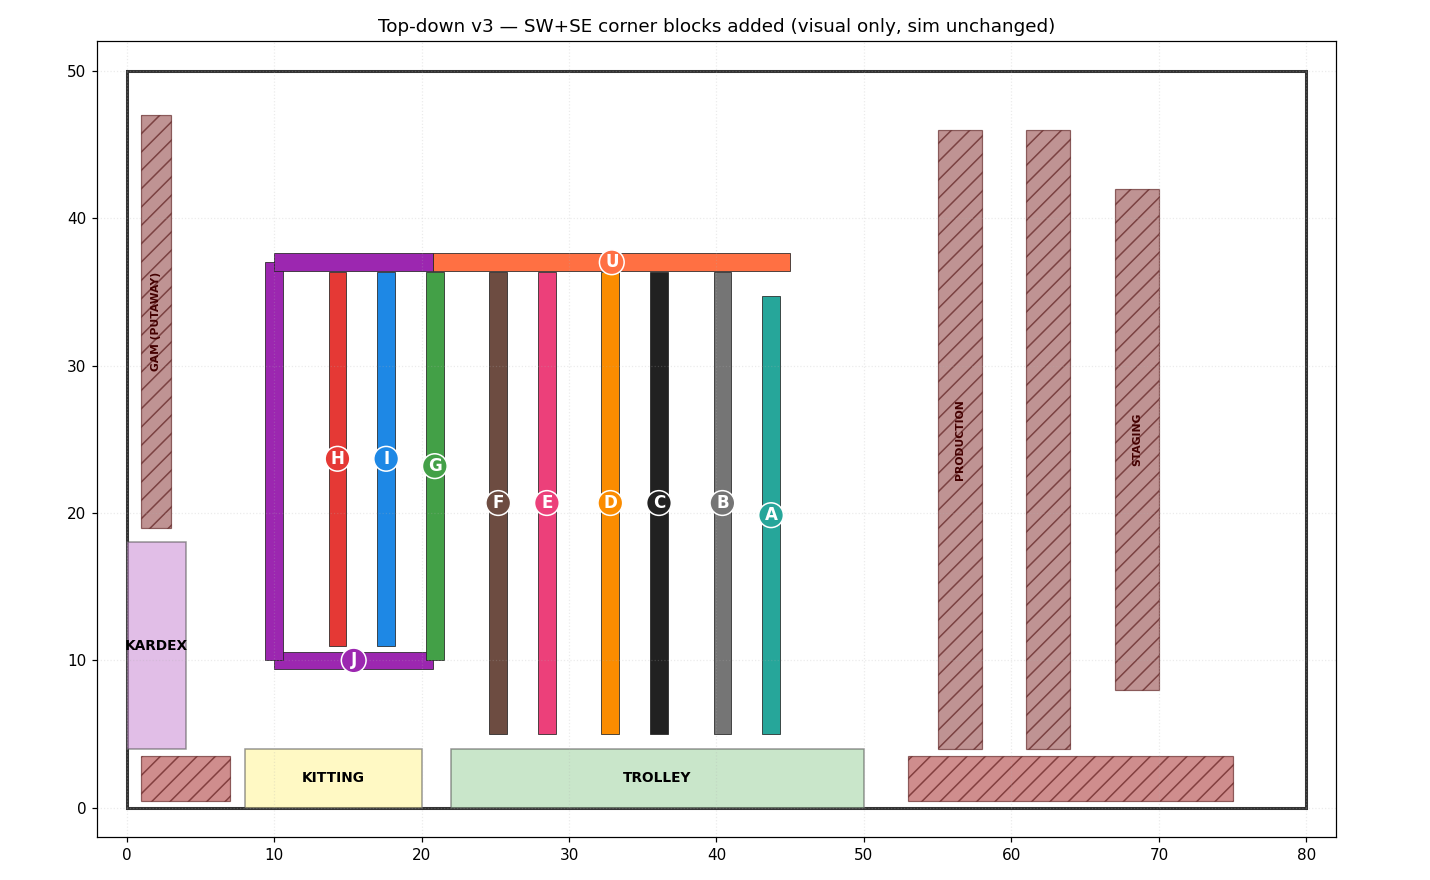
\includegraphics[width=0.92\linewidth]{fig1_layout}\\[3mm]
{\small Modelled warehouse: 11 rack rows (A--J, U); kit corridors alternate with
reach-truck aisles.}
\end{block}

\begin{block}{2.\, Method}
\justifying
A \textbf{discrete-event simulation} (Python / SimPy) driven by \textbf{four
months of real SAP ZWM92 data} (40{,}804 kit orders, 103 active days) and
calibrated with an \textbf{F400 video time-motion study} (2{,}319 micro-events).
Arrivals use empirical batch sizes and gaps; service times are lognormal,
fitted by $\sigma=\sqrt{\ln(1+\mathrm{CV}^{2})}$.
\vspace{4mm}

\textbf{Six storage policies}, all under identical demand ($N=20$, common random
numbers):
\begin{itemize}
\item Baseline -- Actual SAP \, $\cdot$ \, Capacity heuristic
\item Usage-based ABC \, $\cdot$ \, Double ABC \, $\cdot$ \, Travel-distance Optimized
\item \textcolor{segreen!60!black}{\textbf{Line-aware Slotting (proposed)}}
\end{itemize}
\vspace{4mm}

\centering
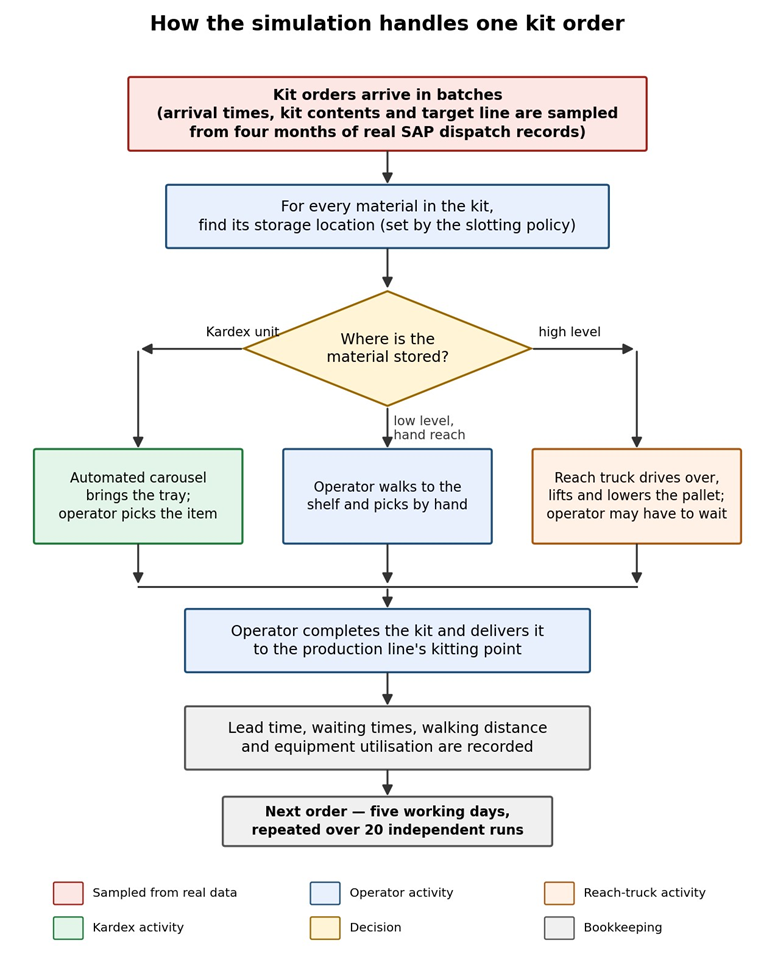
\includegraphics[width=0.74\linewidth]{fig3_lifecycle}\\[3mm]
{\small Lifecycle of one kit order in the model.}
\end{block}
\end{column}

% ---- RIGHT ----
\begin{column}{0.48\textwidth}
\begin{block}{3.\, Results}
\justifying
Across $N=20$ replications, \textbf{Line-aware Slotting} cut mean lead time from
12.37 to \textbf{6.91 min} ($p<0.001$) and reach-truck use from 21.7\% to
\textbf{1.3\%}. Walking distance barely moved (89.0\,$\rightarrow$\,92.4 m), so
the gain comes from \textbf{ending reach-truck queueing}, not shorter walks.
\vspace{5mm}

\centering
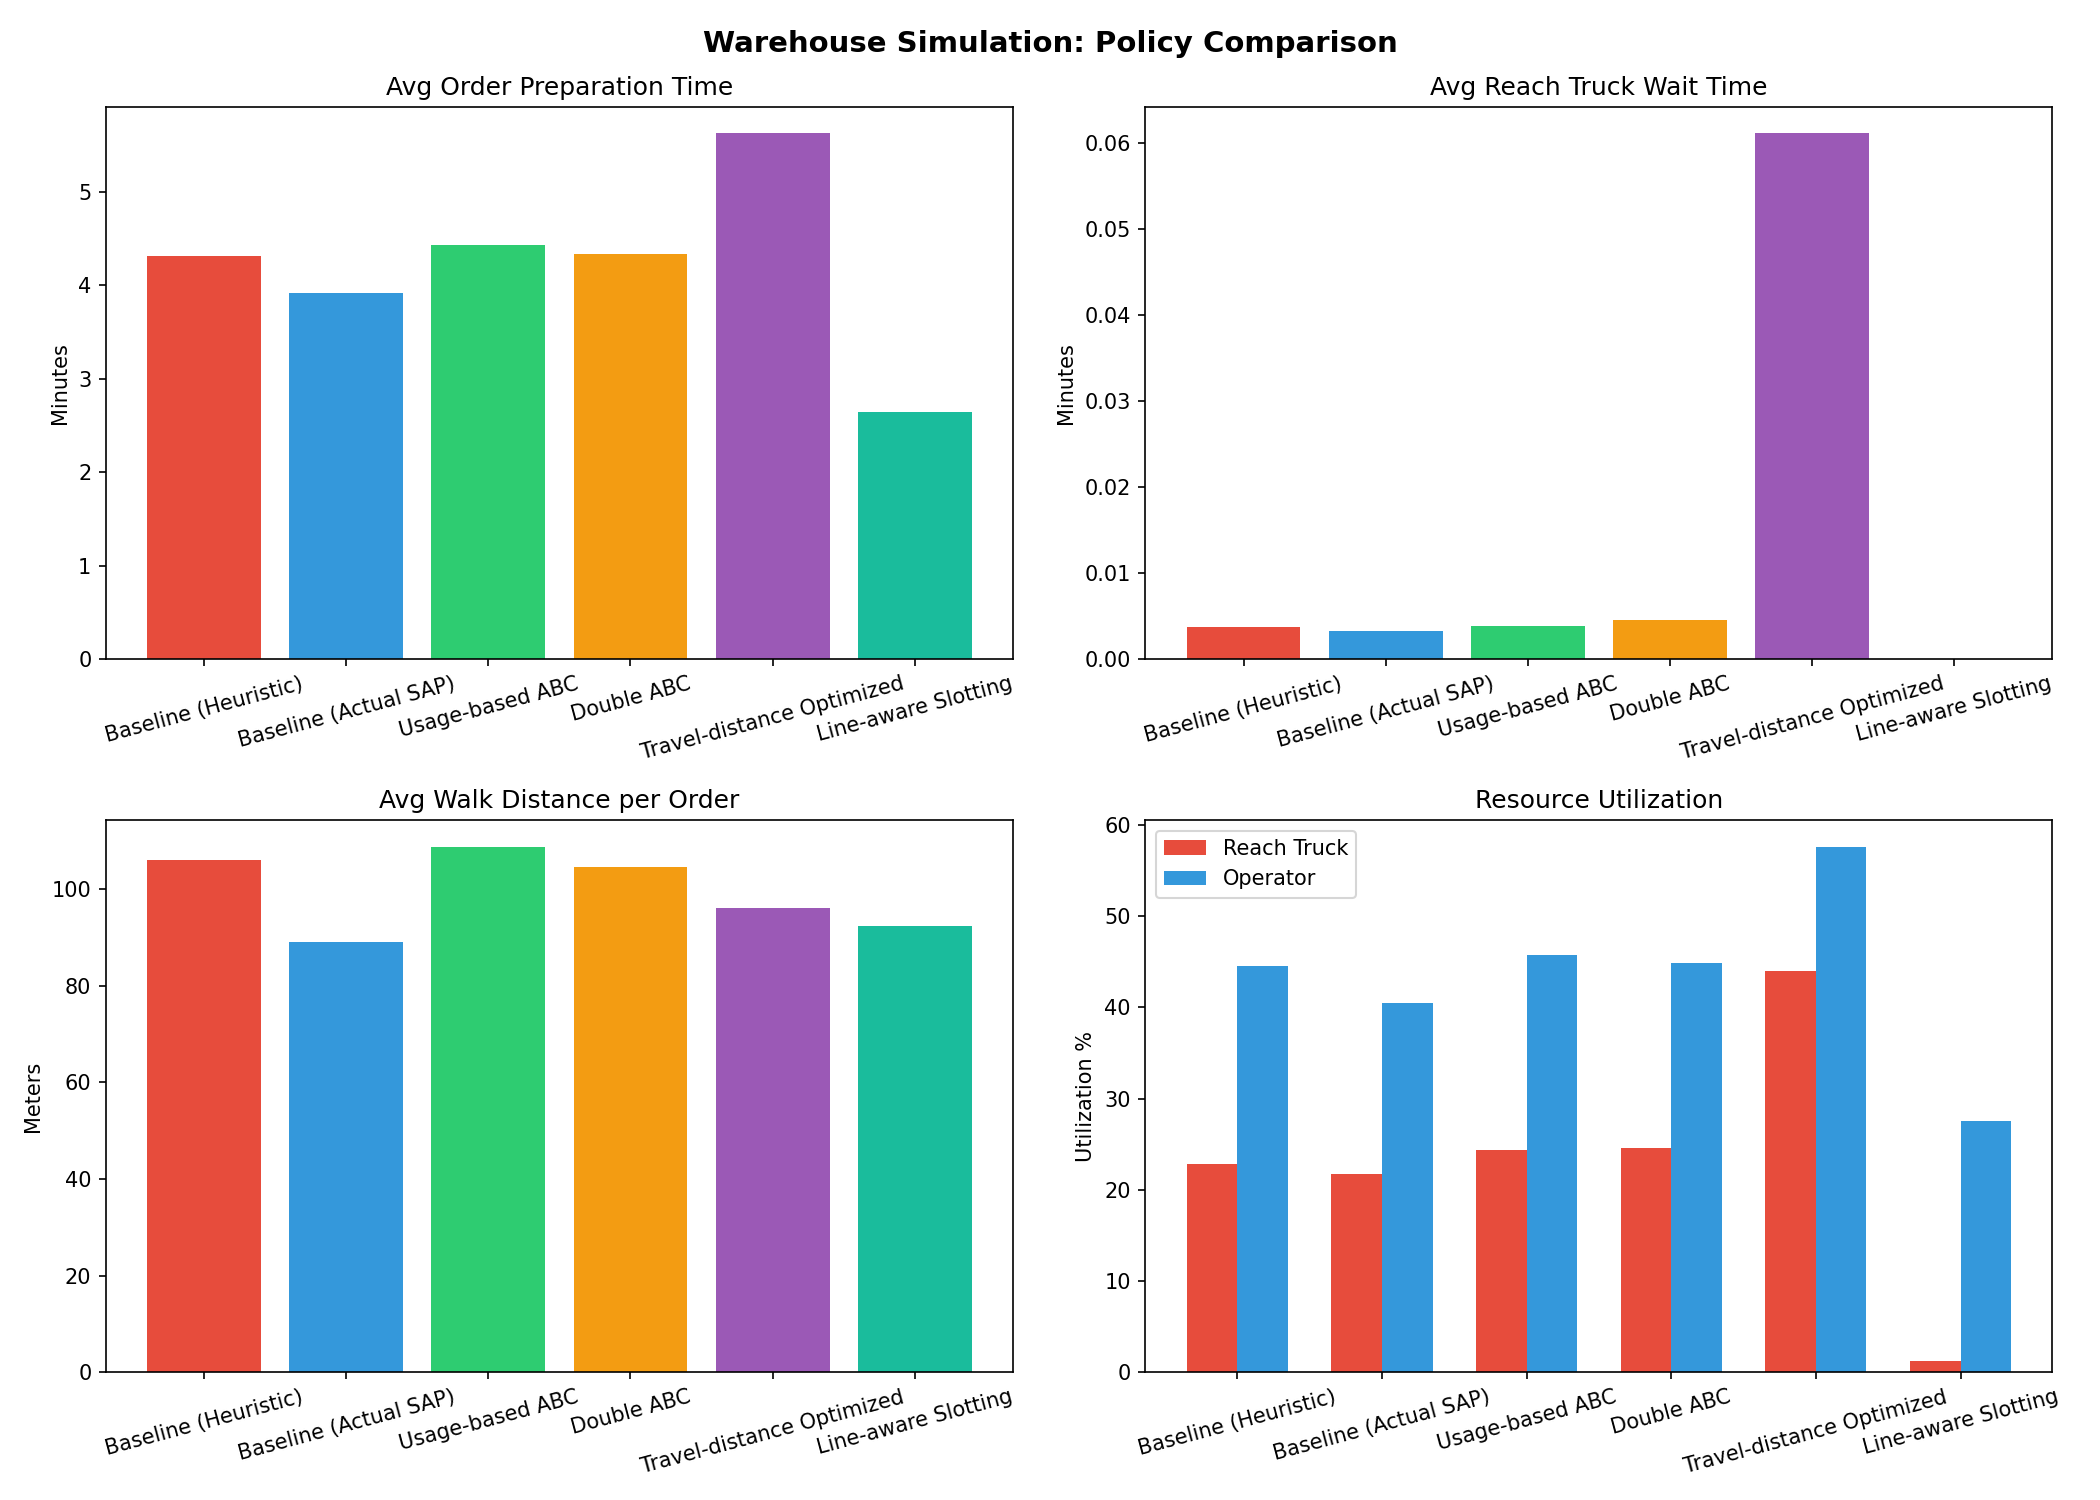
\includegraphics[width=0.97\linewidth]{fig4_comparison}\\[3mm]
{\small Policy comparison across four KPIs.}
\vspace{6mm}

\renewcommand{\arraystretch}{1.25}
\begin{tabular}{lcc}
\toprule
\textbf{Policy} & \textbf{Lead (min)} & \textbf{RT util.} \\
\midrule
\rowcolor{segreen!22}\textbf{Line-aware Slotting} & \textbf{6.91} & \textbf{1.3\%} \\
Baseline (Actual SAP) & 12.37 & 21.7\% \\
Baseline (Heuristic) & 14.71 & 22.8\% \\
Double ABC & 14.74 & 24.6\% \\
Usage-based ABC & 15.24 & 24.4\% \\
Travel-distance Optimized & 24.60 & 44.0\% \\
\bottomrule
\end{tabular}
\end{block}

\begin{block}{4.\, Statistical Evidence}
\justifying
One-way \textbf{ANOVA} rejects equal means for lead time, waiting, utilization
and walk distance ($p<10^{-8}$); throughput is unaffected ($F=0.01$). The CRN
\textbf{paired $t$-test} gives Line-aware vs.\ SAP $=-5.46$ min ($t=-17.47$,
$p=3.7\times10^{-13}$), with effect size \textbf{Cohen's $d=3.10$}. Under a
\textbf{doubled-load stress test} the advantage grows from 5.46 to
\textbf{20.7 min}, so the policy matters most when the system is busiest.
\end{block}

\begin{block}{5.\, Conclusion}
\justifying
Slotting \textbf{line by line} and keeping fast movers at \textbf{hand-reachable
levels} cuts kitting lead time by about \textbf{44\%} and nearly removes
reach-truck dependence, \textbf{with no new equipment and no physical layout
change}. In a kitting warehouse with shared reach trucks, the real lever is
\textbf{resource queueing, not travel distance}.
\end{block}
\end{column}
\end{columns}

\end{frame}
\end{document}
